\documentclass[11pt,a4paper]{article}
\usepackage{fontspec}
\setmainfont{TeX Gyre Termes}
\usepackage[margin=2.4cm]{geometry}
\usepackage{booktabs}
\usepackage{array}
\usepackage{amsmath,amssymb}
\usepackage{microtype}
\usepackage{xcolor}
\usepackage{graphicx}
\usepackage{tikz}
\usetikzlibrary{arrows.meta,positioning,patterns}
\usepackage{pgfplots}
\pgfplotsset{compat=1.18}
\usepackage[hidelinks]{hyperref}
\usepackage{caption}
\captionsetup{font=small,labelfont=bf}
\usepackage{titlesec}
\titleformat{\section}{\normalfont\large\bfseries}{\thesection}{0.6em}{}
\titleformat{\subsection}{\normalfont\normalsize\bfseries}{\thesubsection}{0.6em}{}
\newcolumntype{L}[1]{>{\raggedright\arraybackslash}p{#1}}
\definecolor{cask}{HTML}{2B6CB0}
\definecolor{cstate}{HTML}{8FB8DE}
\definecolor{csilent}{HTML}{C0504D}
\definecolor{cother}{HTML}{BFBFBF}

\title{\vspace{-1.2cm}\bfseries STAR-Clarify: a role-ambiguity benchmark\\
and a clarification skill for language models}
\author{Jean-Jacques Dubray\\[2pt]
\small Cognitive Fab LLC, Kirkland, WA, USA\\
\small \texttt{cto@cognitivefab.com}}
\date{25 November 2026}

\begin{document}
\maketitle

\begin{abstract}
\noindent
A reasoning prompt can state a number without stating what the number is:
``the lift carries 34 people'' gives a capacity or a head count. We call
this the \emph{role} of a value: what the value stands for in the world
the prompt describes. We introduce STAR-Clarify, a benchmark of 396
prompts generated from declared worlds. The expected behavior of each
prompt (answer, ask, or report an impossibility) is set by its
construction, and the answer under each reading is computed. About half of the prompts are clear, so that asking
about everything is penalized. We also describe a short skill, built on
the categories Things, States, Actions and Relationships (STAR), that asks
a model to declare the world of a prompt before reasoning. On the
ambiguous prompts, Claude Opus~5.5 resolves 20\% silently and
Qwen3-30B-A3B 65\%. With the skill these shares fall to 0\% and 13\%. A
control prompt that only tells the model to state its reading, without
STAR, removes most of the silent resolutions (24\% remain), and the skill
keeps its advantage where the role of a value is open, including on verbs
it never names. Asked to judge the wording, the smaller model calls 80\% of
the prompts it resolved silently unclear: it notices most of these
problems and does not report them when it solves.

\medskip\noindent\textbf{Keywords:} large language models; ambiguity;
clarifying questions; underspecified prompts; benchmark; STAR; declared
world; prompt engineering; multilingual prompts
\end{abstract}

\section{Introduction}

A prompt that describes a small world (a puzzle, a plan, a word problem, an
instruction to an agent) gives values and rules. Each value has a
\emph{role}: what it stands for in that world. A role is either a fixed
property of a Thing (the capacity of a jug) or a State that changes (the
water in the jug now). In ``the jug holds 7 litres'', the wording does not
say which: 7 is the size of the jug or the water in it. The answer to a
question about the jug depends on the role chosen
(Figure~\ref{fig:readings}). A person decides from context, and asks when
the context does not decide. A language model also decides, and usually
does not say that it did.

\begin{figure}[t]
\centering
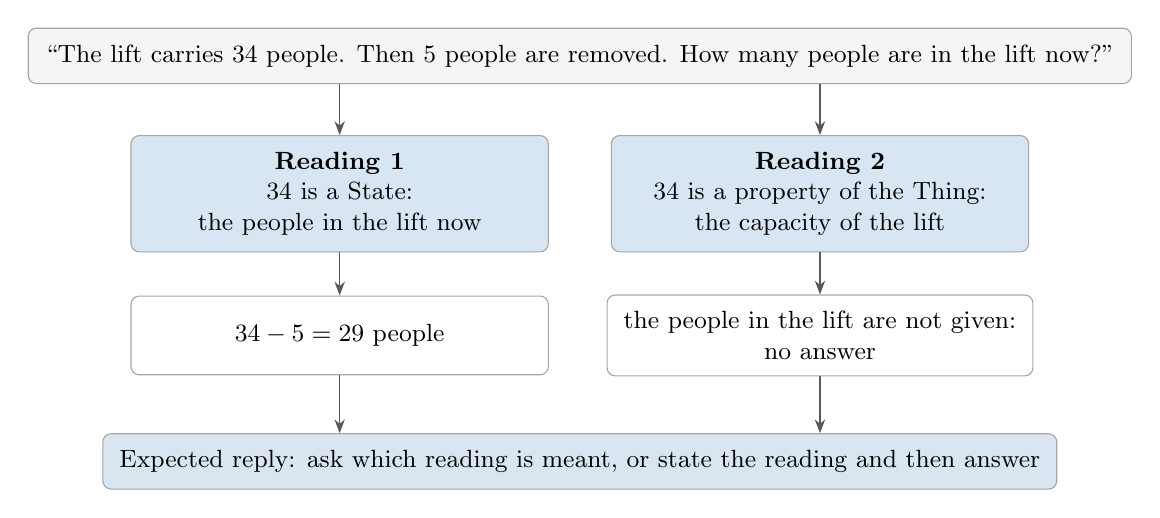
\begin{tikzpicture}[font=\small, box/.style={draw=gray!70, rounded corners=3pt, align=center, inner sep=6pt}, >={Stealth[length=5pt]}]
\node[box, fill=gray!8, minimum width=11.4cm] (p) at (0,0) {``The lift carries 34 people. Then 5 people are removed. How many people are in the lift now?''};
\node[box, fill=cstate!35, minimum width=5.3cm, minimum height=1.45cm] (r1) at (-3.05,-1.75) {\textbf{Reading 1}\\ 34 is a State:\\ the people in the lift now};
\node[box, fill=cstate!35, minimum width=5.3cm, minimum height=1.45cm] (r2) at (3.05,-1.75) {\textbf{Reading 2}\\ 34 is a property of the Thing:\\ the capacity of the lift};
\node[box, minimum width=5.3cm, minimum height=1.0cm] (a1) at (-3.05,-3.55) {$34-5=29$ people};
\node[box, minimum width=5.3cm, minimum height=1.0cm] (a2) at (3.05,-3.55) {the people in the lift are not given:\\ no answer};
\node[box, fill=cask!18, minimum width=11.4cm] (e) at (0,-5.15) {Expected reply: ask which reading is meant, or state the reading and then answer};
\draw[->, gray!70!black] (p.south -| r1.north) -- (r1.north);
\draw[->, gray!70!black] (p.south -| r2.north) -- (r2.north);
\draw[->, gray!70!black] (r1) -- (a1);
\draw[->, gray!70!black] (r2) -- (a2);
\draw[->, gray!70!black] (a1.south) -- (a1.south |- e.north);
\draw[->, gray!70!black] (a2.south) -- (a2.south |- e.north);
\end{tikzpicture}
\caption{One prompt, two roles for the same number. The two readings give
different answers, so the prompt is expected to be clarified.}
\label{fig:readings}
\end{figure}

Two results motivate this study. A study of the reasoning traces of four
models on water-jug problems \cite{dubray2026grammarllm} described every
sentence of the reasoning with four categories of human language (Things,
States, Actions, Relationships: STAR), and found that errors start in one
category. When a French translation used ``contient'' for a capacity,
open-weight models read the capacity as the current contents. When a
Chinese translation narrowed a rule worded with ``only'', the errors moved
to that rule. No model asked what the wording meant. An intervention on
two open-weight models then showed that the role of a number is carried by
the words around it, and that exchanging the roles changes the answer.

These results suggest a practical remedy: before reasoning, write down the
Things, States, Actions and Relationships of the prompt, give every value
its role, and ask when a value or a rule has two readings. This paper
tests that remedy. It contributes:

\begin{itemize}\setlength\itemsep{2pt}
\item a benchmark, STAR-Clarify, of 396 prompts with exact expected
behavior, half of them clear, and two additional sets (held-out verbs,
and triples that differ only in the form of the verb);
\item a skill (a system prompt of about 1,200 words) that applies the STAR
declaration, with two variants and a control prompt without STAR;
\item a measurement on one frontier model and one open-weight model, with
a recognition probe that separates noticing an ambiguity from acting on
it.
\end{itemize}

The scope of the study is limited. Two models were tested, the labels of
the benchmark come from the author, and the judge of free-text replies is
a third model. Section~\ref{sec:limits} lists what follows from these
choices.

\section{Related work}

\paragraph{Asking for missing information.}
QuestBench \cite{li2025questbench} frames clarification as a constraint
problem with one missing variable, in logic, planning and arithmetic, and
asks the model to select the right question among several. Models that
solve the fully specified problem often fail to pick the question.
AskBench \cite{zhao2026askbench} turns question answering into multi-turn
exchanges and scores when and what a model asks. CLAMBER
\cite{zhang2024clamber} proposes a taxonomy of ambiguous queries and finds
that models rarely produce useful clarifying questions. Su and Cardie
\cite{su2026knowing} separate recognition from behavior: models identify
an ambiguity when asked to judge it, and answer directly when they are
not. STAR-Clarify measures the same gap on reasoning prompts with state,
and tests a remedy.

\paragraph{Ambiguity in language.}
AmbiEnt \cite{liu2023afraid} is a linguist-annotated set of ambiguous
sentences, on which models struggle to recognize and separate the
readings. Its ambiguities are those of general language. Ours are narrower:
a value whose role is open, a rule whose scope is open, a reference with
two candidates.

\paragraph{Underspecified prompts.}
Yang et al. \cite{yang2026prompts} study prompts written by developers and
show that models guess unspecified requirements correctly less than half
of the time, and that the guesses change across model versions. The skill
studied here is a way to make a prompt's requirements explicit before a
model reasons over it.

\paragraph{Irrelevant context.}
GSM-IC \cite{shi2023distracted} adds one irrelevant sentence to arithmetic
problems and shows that it changes the answers. STAR-Clarify includes
distractors, some with a role-ambiguous verb on a Thing the question does
not use.

\paragraph{Roles inside models.}
Feng and Steinhardt \cite{feng2024binding} show that models bind entities
to attributes with identifiable vectors. Li and Webb
\cite{li2026symbolic} show that mechanisms which treat tokens as abstract
variables emerge in sequence tasks when the training data is diverse. The
STAR categories draw on the ontological categories of conceptual semantics
\cite{jackendoff1990semantic}, which is a larger set. None of this work
tests a fixed property against a changing state of the same Thing, which
is the case the benchmark is built around.

\section{The benchmark}
\label{sec:bench}

\subsection{Generation from declared worlds}

Each prompt is produced by a program from a declared world: a small set of
Things with fixed properties, States with starting values, Actions with
preconditions and effects, and Relationships. The program varies the
numbers, the wording, the order of the sentences and the language. Because
the world is a program, the expected behavior of each prompt and its
answer under each reading are computed, not annotated. Planning answers
(the smallest number of actions) come from a breadth-first search.

\subsection{Definition of an ambiguous prompt}

A prompt is \emph{ambiguous} when two declared worlds fit its text and
give different answers to its question. The two worlds are its
\emph{readings}. A question \emph{resolves} the prompt when its answer
leaves one world. For a value whose role is open, the two worlds differ by
one assignment: the number is a property of the Thing in one, and a State
in the other. When two worlds fit the text and give the same answer, the
prompt is not ambiguous for that question, and asking is needless. A
\emph{missing} quantity is a different case: one world fits, and a value
that its answer needs is absent, which is the setting of QuestBench
\cite{li2025questbench}.

\subsection{Categories}

Table~\ref{tab:cats} lists the ten categories. Four expected behaviors
are used: \emph{answer} (191 prompts), \emph{clarify} (125: ask a
question, or answer after stating the reading), \emph{missing} (43: ask
for a value) and \emph{impossible} (37: say that the goal cannot be
reached, or name a contradiction). English accounts for 320 prompts,
French 32, Spanish 22, German 20 and Chinese 2.

\begin{table}[t]
\centering\small
\begin{tabular}{@{}l L{4.1cm} r L{2.0cm} L{6.0cm}@{}}
\toprule
& Category & $n$ & Expected & Example \\
\midrule
C1 & Clear property and state, ten domains & 50 & answer & The tank can take at most 48 litres. The tank has 33 litres of fuel in it right now. How many more litres can be added? \\
C2 & Role-ambiguous verb & 40 & clarify & The lift carries 34 people. Then 5 people are removed. How many people are in the lift now? \\
C3 & Same verb for property and state (EN, FR, ES, DE; both orders) & 60 & clarify & La cruche A contient exactement 8 litres. En ce moment, la cruche A contient 3 litres d'eau. \\
C4 & Rules worded with ``only'' & 33 & clarify or answer & Water can only be poured from jug X or jug Y into jug Z or jug T. Is it allowed to pour water from jug X into jug Y? \\
C5 & Irreversible store & 30 & answer or impossible & Water poured into the store can never be taken back. Smallest number of actions for exactly $g$ litres in the store? \\
C6 & Missing quantity & 43 & missing & A shop sells pens in boxes. Maria buys 12 boxes. How many pens does she have? \\
C7 & Irrelevant sentence & 40 & answer & A second jug on the shelf contains 9 litres. \\
C8 & Unreachable goal, contradiction & 30 & impossible & Jug A can hold at most 6 litres. Jug A has 16 litres of water in it right now. \\
C9 & Reference with two candidates & 30 & clarify or answer & Jug A is poured into jug B, and then it has 3 litres of water in it. \\
C10 & Clear planning (EN, FR, ES, DE) & 40 & answer & Smallest number of actions that leaves exactly $g$ litres in one of the jugs? \\
\bottomrule
\end{tabular}
\caption{The ten categories of STAR-Clarify. C4 and C9 mix ambiguous
prompts with clear controls.}
\label{tab:cats}
\end{table}

\subsection{Relation to known types of ambiguity}

Most categories are instances of types that earlier benchmarks already
name (Table~\ref{tab:types}). The case that is specific to this benchmark
is the value whose role is open: the same sentence states a fixed property
or a changing state of one Thing. In English this is a property of the
simple present (``carries 34 people'' states what is the case now, or what
the lift can do), more than of any single verb.

\begin{table}[t]
\centering\small
\begin{tabular}{@{}l L{4.4cm} L{4.6cm} L{4.0cm}@{}}
\toprule
& Category & Known type & Closest earlier work \\
\midrule
C2, C3 & Value whose role is open & Lexical ambiguity of the verb, between a property and a state & none for this contrast \\
C4 & Rules worded with ``only'' & Scope ambiguity & AmbiEnt \cite{liu2023afraid} \\
C9 & Reference with two candidates & Referential ambiguity & CLAMBER \cite{zhang2024clamber} \\
C6 & Missing quantity & Missing information & QuestBench \cite{li2025questbench}, AskBench \cite{zhao2026askbench} \\
C8 & Unreachable goal, contradiction & Contradiction in the prompt & CLAMBER \cite{zhang2024clamber} \\
C7 & Irrelevant sentence & Distractor & GSM-IC \cite{shi2023distracted} \\
C5 & Irreversible store & Not an ambiguity: tracking of a state that cannot be undone & \\
C1, C10 & Clear prompts & Controls & \\
\bottomrule
\end{tabular}
\caption{The categories of STAR-Clarify against known types of ambiguity.}
\label{tab:types}
\end{table}

\subsection{Controls against over-asking}

A model that asks about every prompt would score well on the ambiguous
ones. Three kinds of control prevent this. C1, C7 and C10 are clear. C4
and C9 pair each ambiguous prompt with a reworded clear one. C4 also
contains rules whose two readings give the same answer to the question
asked: a question there is counted as needless.

\subsection{Two additional sets}
\label{sec:sets}

Two sets were added to test the main result on role ambiguity.

\emph{Held-out verbs} (80 prompts). The 40 ambiguous prompts use the
template of C2 with eight verbs and Things that appear in no version of
the skill and in no prompt of the benchmark (stocks, houses, hosts,
transports, shelters, keeps, accommodates, admits). The other 40 are clear
controls on the same Things.

\emph{Verb-form triples} (120 prompts). The template of C2 ends with
``Then 5 people are removed'', which presupposes that people are in the
lift and so favors one reading. In the triples the question follows the
statement directly, and only the form of the verb changes
(Table~\ref{tab:triples}).

\begin{table}[t]
\centering\small
\begin{tabular}{@{}L{2.6cm} L{8.2cm} L{4.0cm}@{}}
\toprule
Form & Prompt & Expected \\
\midrule
Simple present & The lift carries 34 people. How many people are in the lift right now? & ask, or state the reading \\
Progressive & The lift is carrying 34 people right now. How many people are in the lift right now? & answer 34 \\
Modal & The lift can carry at most 34 people. How many people are in the lift right now? & report that the number is not given \\
\bottomrule
\end{tabular}
\caption{One verb-form triple. Eight Things, five numbers each.}
\label{tab:triples}
\end{table}

\section{The skill}
\label{sec:skill}

The skill is a text of about 1,200 words given as a system prompt. Its
procedure has five steps. In what follows, ``the skill'' is this first
version.

\begin{enumerate}\setlength\itemsep{2pt}
\item \textbf{Declare the world as a STAR table.} List the Things with
their fixed properties, the States with their starting values, the Actions
with preconditions and effects, and the Relationships and the goal. Keep
fixed properties apart from changing states. Write the role of every value
next to it.
\item \textbf{Check each value and rule for a second reading.} The skill
lists the wordings to check: verbs that can state a capacity or a current
amount (holds, contains, has, takes, carries, ``contient''), the same word
used for two roles, rules with ``only'', translated wording, and anything
that cannot be undone.
\item \textbf{Ask, or state the reading.} Ask one short question that
names the two readings. If nobody can be asked, state the reading chosen
at the top of the answer. Never resolve an ambiguity silently.
\item \textbf{Rewrite the prompt}, when the task is to write one.
\item \textbf{Reason against the declaration}, one Action and resulting
State per step, then check the answer category by category.
\end{enumerate}

\paragraph{Version 2.} Version~2 adds rules for missing values,
contradictions, unclear references and irrelevant facts, and the rule
``ask only when the readings lead to different answers''. It was written
after the benchmark categories.

\paragraph{Version 3.} Version~3 replaces the list of wordings with a
structural test: fill the slots of the STAR structure that the question
needs, and ask only when a slot is empty, a value fits two slots, or a
rule does not say what holds outside the cases it covers.

\paragraph{Control prompt.} The control is a system prompt of similar
length (about 900 words) that gives general advice on careful reading and
keeps step~3 word for word: ask, or state the reading, and never resolve
an ambiguity silently. It has no STAR table, no distinction between
properties and states, and no list of wordings.

\section{Method}

Figure~\ref{fig:protocol} shows the path of one prompt.

\begin{figure}[!htb]
\centering
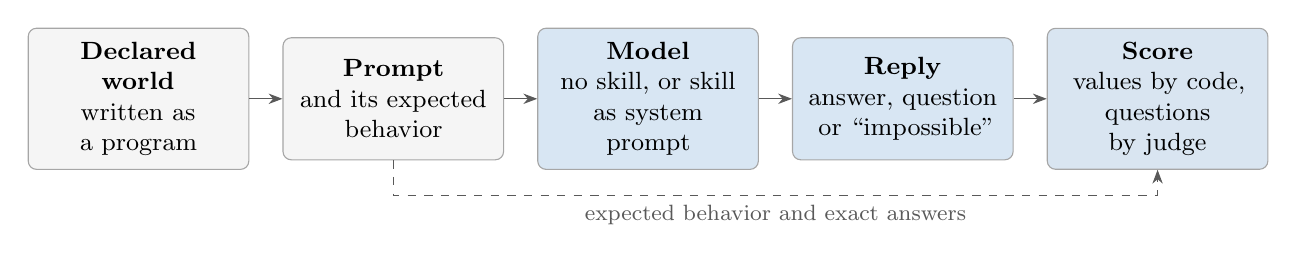
\begin{tikzpicture}[font=\small, box/.style={draw=gray!70, rounded corners=3pt, align=center, inner sep=5pt, text width=2.45cm, minimum height=1.55cm}, >={Stealth[length=5pt]}, node distance=0.42cm]
\node[box, fill=gray!8] (w) {\textbf{Declared world}\\ written as\\ a program};
\node[box, fill=gray!8, right=of w] (p) {\textbf{Prompt}\\ and its expected\\ behavior};
\node[box, fill=cstate!35, right=of p] (m) {\textbf{Model}\\ no skill, or skill\\ as system prompt};
\node[box, fill=cstate!35, right=of m] (r) {\textbf{Reply}\\ answer, question\\ or ``impossible''};
\node[box, fill=cask!18, right=of r] (s) {\textbf{Score}\\ values by code,\\ questions by judge};
\draw[->, gray!70!black] (w) -- (p);
\draw[->, gray!70!black] (p) -- (m);
\draw[->, gray!70!black] (m) -- (r);
\draw[->, gray!70!black] (r) -- (s);
\draw[->, gray!70!black, dashed] (p.south) -- ++(0,-0.45) -| node[pos=0.25, below, font=\footnotesize] {expected behavior and exact answers} (s.south);
\end{tikzpicture}
\caption{The path of one prompt. The expected behavior and the answers
are computed by the program that generates the prompt, and are compared
with the reply at the end.}
\label{fig:protocol}
\end{figure}

\paragraph{Models.}
Claude Opus~5.5 was called through the Anthropic API with default sampling.
Qwen3-30B-A3B (thinking variant, 4-bit quantized) was served with
llama.cpp on GPUs, with the sampling settings of its model card
(temperature 0.6, top-p 0.95, top-k 20). Its reasoning tokens were
discarded and only the final content was scored.

\paragraph{Conditions.}
\emph{No skill}: no system prompt. \emph{Skill}, \emph{version~2},
\emph{control}: the corresponding text as system prompt. Opus was run
without the skill, with the skill and with version~2. Qwen3 was run in
all four conditions on the 396 prompts and on the held-out verbs, and
without version~2 on the triples. Version~3 was run on Qwen3 on 100
prompts.

\paragraph{Reply format.}
In the main runs every prompt ends with the same instruction: ``If you
need to ask me a question before you can answer, ask it'', followed by a
request to end with one line that starts with \texttt{FINAL:} and gives
an answer, a question (\texttt{ASK:}) or an impossibility
(\texttt{IMPOSSIBLE:}). Two other endings were tested on Qwen3: one that
only asks for the final line (\emph{no invitation}), and one that says
``Nobody is available to answer questions: give your best answer now''
(\emph{nobody to ask}).

\paragraph{Scoring.}
Numbers and yes/no answers are checked by code against the computed
answer. For prompts expected to be clarified, a reply receives credit if
it asks about the ambiguity in the prompt, or if it states in words the
reading it adopts and its answer is right under that reading. A reply that
follows one reading without saying so is a \emph{silent resolution} and
receives no credit, even when its number matches a reading. A question
and a stated reading are different acts. A question acquires information.
A stated reading does not, but it lets the reader correct the choice, and
it is the only option when nobody can be asked. Both receive credit, and
they are reported separately (Table~\ref{tab:acts}). For missing
quantities, asking for the quantity receives credit, a stated assumption
half credit, and a silent guess none. A second model, Mistral Large,
judges one thing only: whether the question or the stated reading concerns
the known issue of the prompt. Every verdict was readable in the reported
runs. The same replies judged three times gave 89.6\%, 87.2\% and 88.8\%
of ambiguities handled, so differences of about two points are within the
precision of the judge. Conditions are compared on the same prompts with a
two-sided sign test.

\paragraph{Recognition probe.}
In a separate condition the model does not solve the prompt. It is asked
whether a value, a rule or a reference can be read in two ways that lead
to different answers, whether a needed value is missing, or whether two
statements conflict, and it ends with \texttt{FINAL: CLEAR} or
\texttt{FINAL: UNCLEAR}. This is scored by code.

\section{Results}

Three terms are used throughout. A prompt expected to be clarified is
\emph{handled} when the reply asks about its ambiguity or states the
reading it takes. It is \emph{resolved silently} when the reply follows
one reading without saying so. \emph{Credit} is 1 for a correct or
handled reply, 0.5 for a stated assumption on a missing quantity, and 0
otherwise.

One result qualifies the others and is given first. The role-ambiguous
prompts of the benchmark continue with a sentence that favors one
reading. Without that sentence the smaller model handles 62\% of them
unaided, and 0\% with it (Section~\ref{sec:triples}).

\subsection{Baseline and effect of the skill}

\subsubsection{Silent resolution without the skill}

Without the skill, both models answer the clear prompts correctly (Opus
97\%, Qwen3 95\%) and ask for missing quantities (100\% for both, counting
replies that declare the problem unanswerable). This last result holds
for an easy case: one value is missing from a one-step problem, and the
prompt invites a question. It says little about harder problems. They differ on the 125
prompts expected to be clarified (Figure~\ref{fig:outcomes}).

Opus states its reading unprompted on 84 of them and asks on 16. It
resolves 25 silently (20\%): 17 role-ambiguous verbs and 8 rules with
``only''. On the 60 prompts that use the same verb for a property and a
state, in four languages, it states on 50 that it takes the ``exactly''
sentence as the capacity, and asks on the other 10.

Qwen3 resolves 81 silently (65\%). It asks on 2. On role-ambiguous verbs
its credit is 0.00: ``The lift carries 34 people. Then 5 people are
removed'' is answered 29 without comment. On the same-verb prompts the
order of the sentences matters. When the property sentence comes first,
credit is 0.20. When the state sentence comes first, credit is 0.80,
mostly because the model reports a conflict between two values for the
contents. The same order effect appeared inside this model in the earlier
study \cite{dubray2026grammarllm}.

\begin{figure}[t]
\centering
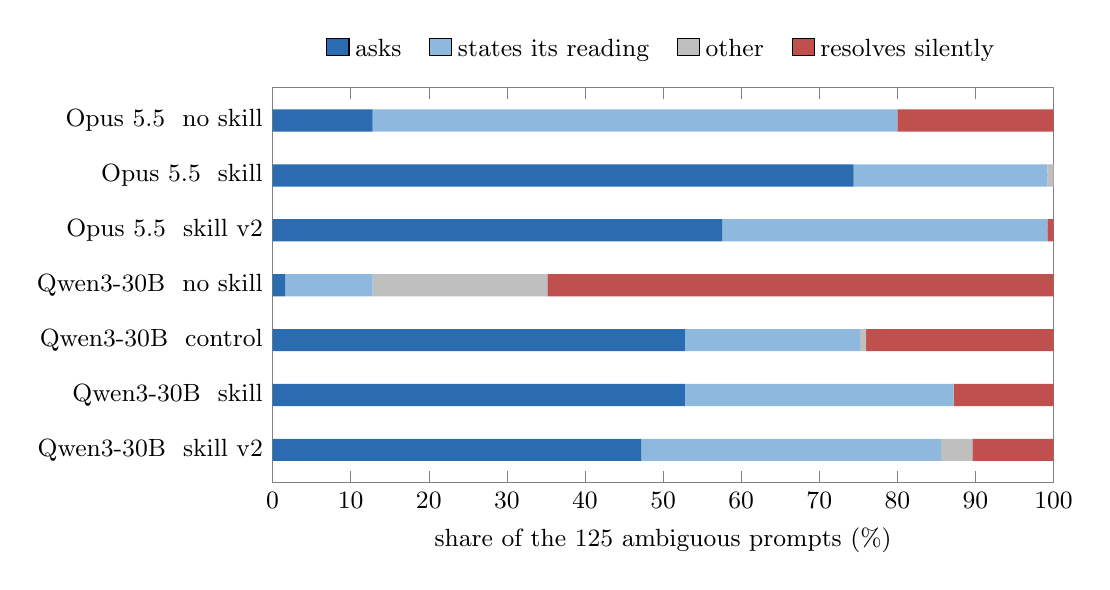
\begin{tikzpicture}
\begin{axis}[
  xbar stacked, width=11.5cm, height=6.6cm, bar width=8pt,
  xmin=0, xmax=100, xlabel={\small share of the 125 ambiguous prompts (\%)},
  ytick=data, y dir=reverse,
  yticklabels={Opus 5.5\ \ no skill, Opus 5.5\ \ skill, Opus 5.5\ \ skill v2, Qwen3-30B\ \ no skill, Qwen3-30B\ \ control, Qwen3-30B\ \ skill, Qwen3-30B\ \ skill v2},
  yticklabel style={font=\small}, xticklabel style={font=\small},
  legend style={at={(0.5,1.04)},anchor=south,legend columns=4,font=\small,draw=none,/tikz/every even column/.append style={column sep=8pt}},
  axis line style={gray}, tick style={gray}, enlarge y limits=0.10,
]
\addplot[fill=cask,draw=none] coordinates {(12.8,0) (74.4,1) (57.6,2) (1.6,3) (52.8,4) (52.8,5) (47.2,6)};
\addplot[fill=cstate,draw=none] coordinates {(67.2,0) (24.8,1) (41.6,2) (11.2,3) (22.4,4) (34.4,5) (38.4,6)};
\addplot[fill=cother,draw=none] coordinates {(0,0) (0.8,1) (0,2) (22.4,3) (0.8,4) (0,5) (4.0,6)};
\addplot[fill=csilent,draw=none] coordinates {(20.0,0) (0,1) (0.8,2) (64.8,3) (24.0,4) (12.8,5) (10.4,6)};
\legend{asks, states its reading, other, resolves silently}
\end{axis}
\end{tikzpicture}
\caption{What each model does on the 125 prompts expected to be clarified.
``Other'' groups replies that report a conflict between two statements
(credited when on target), questions and stated readings that miss the
issue, and replies without a final line.}
\label{fig:outcomes}
\end{figure}

\begin{table}[t]
\centering\small
\begin{tabular}{@{}l l rrrr r r@{}}
\toprule
& & \multicolumn{4}{c}{Of the 125 ambiguous prompts} & & \\
\cmidrule(lr){3-6}
Model & Condition & asked & stated & conflict & silent, other & Handled & Precision \\
\midrule
Opus 5.5 & no skill & 16 & 84 & 0 & 25 & 80.0\% & 0.84 \\
& skill & 93 & 31 & 0 & 1 & 99.2\% & 0.94 \\
& version 2 & 72 & 52 & 0 & 1 & 99.2\% & 0.96 \\
\midrule
Qwen3-30B-A3B & no skill & 2 & 14 & 23 & 86 & 31.2\% & 0.67 \\
& control & 66 & 28 & 1 & 30 & 76.0\% & 0.93 \\
& skill & 66 & 43 & 0 & 16 & 87.2\% & 0.89 \\
& version 2 & 59 & 48 & 5 & 13 & 89.6\% & 0.97 \\
\bottomrule
\end{tabular}
\caption{Questions and stated readings, reported separately. ``Handled''
is the share of the 125 ambiguous prompts with a question, a stated
reading or a reported conflict on target (recall). ``Precision of
questions'' is the share of all questions asked on ambiguous and clear
prompts that fall on an ambiguous prompt and on its issue.}
\label{tab:acts}
\end{table}

\subsubsection{Effect of the skill}

With the skill, silent resolution falls from 20\% to 0\% for Opus and from
65\% to 13\% for Qwen3 (Table~\ref{tab:main}). The skill is better than no
skill on 25 prompts and worse on 3 for Opus, and better on 80 and worse on
11 for Qwen3 (sign test $p<0.0001$ for both).

The gain is concentrated where the earlier study located the errors
(Table~\ref{tab:cat}). On role-ambiguous verbs, credit rises from 0.57 to
1.00 for Opus and from 0.00 to 0.88 for Qwen3. On the same-verb prompts,
Qwen3 rises from 0.50 to 1.00, and reaches 1.00 in each of the four
languages.

The skill also changes the form of the reply. Without it, Opus mostly
states a reading and answers. With it, Opus mostly asks (93 questions
against 16).

Version~2 handles as many ambiguities as the skill: the two are within
the precision of the judge on both models. Its main effect is on needless
questions: 3 against 6 for Opus, and 2 against 8 for Qwen3. Its replies
are also shorter. Because version~2 was written after the benchmark categories, this
result needs a confirmation on prompts written by someone else.

\begin{table}[t]
\centering\small
\begin{tabular}{@{}L{4.6cm} rrr @{\hspace{1.0em}} rrrr@{}}
\toprule
& \multicolumn{3}{c}{Opus 5.5} & \multicolumn{4}{c}{Qwen3-30B-A3B} \\
\cmidrule(lr){2-4}\cmidrule(l){5-8}
Measure & no skill & skill & v2 & no skill & control & skill & v2 \\
\midrule
Ambiguity handled (asked, or reading stated), $n=125$ & 80.0\% & 99.2\% & 99.2\% & 31.2\% & 76.0\% & 87.2\% & 89.6\% \\
Ambiguity resolved silently & 20.0\% & 0.0\% & 0.8\% & 64.8\% & 24.0\% & 12.8\% & 10.4\% \\
Clear prompts answered correctly, $n=191$ & 97.4\% & 96.3\% & 97.9\% & 95.3\% & 96.3\% & 93.7\% & 95.3\% \\
Needless questions on clear prompts & 1.6\% & 3.1\% & 1.6\% & 0.5\% & 2.6\% & 4.2\% & 1.0\% \\
Missing quantity asked for, $n=43$ & 100\% & 100\% & 100\% & 100\% & 100\% & 100\% & 100\% \\
Impossible or contradictory detected, $n=37$ & 100\% & 100\% & 100\% & 91.9\% & 91.9\% & 97.3\% & 100\% \\
Mean credit, $n=396$ & 0.924 & 0.980 & 0.987 & 0.753 & 0.899 & 0.927 & 0.944 \\
Better / worse than no skill & & 25 / 3 & 27 / 2 & & 66 / 8 & 80 / 11 & 83 / 7 \\
Mean output tokens & 380 & 915 & 783 & 1,695 & 2,330 & 3,882 & 3,546 \\
\bottomrule
\end{tabular}
\caption{Results on the 396 prompts. Output tokens exclude the reasoning
tokens of Qwen3.}
\label{tab:main}
\end{table}

\begin{table}[t]
\centering\small
\begin{tabular}{@{}l L{4.6cm} r rrr @{\hspace{1.0em}} rrrr@{}}
\toprule
& & & \multicolumn{3}{c}{Opus 5.5} & \multicolumn{4}{c}{Qwen3-30B-A3B} \\
\cmidrule(lr){4-6}\cmidrule(l){7-10}
& Category & $n$ & no skill & skill & v2 & no skill & control & skill & v2 \\
\midrule
C1 & Clear property and state & 50 & 1.00 & 1.00 & 1.00 & 1.00 & 0.96 & 0.96 & 0.98 \\
C2 & Role-ambiguous verb & 40 & 0.57 & 1.00 & 1.00 & 0.00 & 0.60 & 0.88 & 0.88 \\
C3 & Same verb for property and state & 60 & 1.00 & 1.00 & 1.00 & 0.50 & 0.97 & 1.00 & 1.00 \\
C4 & Rules worded with ``only'' & 33 & 0.64 & 0.79 & 0.88 & 0.61 & 0.67 & 0.64 & 0.76 \\
C5 & Irreversible store & 30 & 1.00 & 0.97 & 1.00 & 0.93 & 0.90 & 0.87 & 0.90 \\
C6 & Missing quantity & 43 & 1.00 & 1.00 & 1.00 & 1.00 & 1.00 & 1.00 & 1.00 \\
C7 & Irrelevant sentence & 40 & 0.97 & 1.00 & 1.00 & 0.93 & 0.95 & 0.95 & 0.95 \\
C8 & Unreachable goal, contradiction & 30 & 1.00 & 1.00 & 1.00 & 0.90 & 0.93 & 0.97 & 1.00 \\
C9 & Reference with two candidates & 30 & 1.00 & 1.00 & 1.00 & 0.77 & 0.93 & 0.90 & 0.97 \\
C10 & Clear planning & 40 & 1.00 & 1.00 & 0.97 & 1.00 & 1.00 & 1.00 & 0.95 \\
\bottomrule
\end{tabular}
\caption{Mean credit by category.}
\label{tab:cat}
\end{table}

\subsection{Checks on the main result}

\subsubsection{Control prompt without STAR}

The control prompt answers one question: how much of the effect comes from
the instruction to state a reading, and how much from the STAR
declaration. On Qwen3 the control handles 76\% of the ambiguous prompts,
against 31\% without a system prompt and 87\% with the skill
(Table~\ref{tab:main}). A prompt without STAR that keeps the instruction
therefore produces most of the gain. The control also contains general
advice on careful reading, so this is an upper bound on what the
instruction does alone. Over the 396 prompts the skill is better than the control on 25
prompts and worse on 14 ($p=0.11$), and version~2 is better on 28 and
worse on 10 ($p=0.005$).

The difference between the control and the skill is not spread evenly. It
sits on the values whose role is open (Figure~\ref{fig:roles}): 0.60
against 0.88 on role-ambiguous verbs. On the same-verb prompts, the
references and the ``only'' rules the control does as well as the skill.
The control also writes shorter replies (2,330 tokens against 3,882).

\begin{figure}[t]
\centering
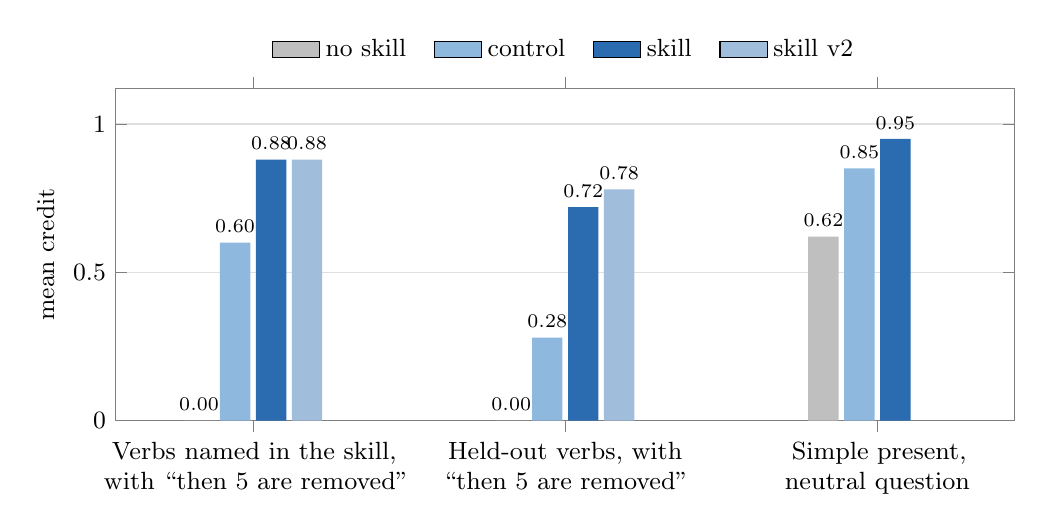
\begin{tikzpicture}
\begin{axis}[
  ybar, area legend, width=13.0cm, height=5.8cm, bar width=11pt,
  ymin=0, ymax=1.12, ylabel={\small mean credit},
  symbolic x coords={C2,H2,N2}, xtick=data,
  xticklabels={{Verbs named in the skill, with ``then 5 are removed''},{Held-out verbs, with ``then 5 are removed''},{Simple present, neutral question}},
  xticklabel style={font=\small, text width=3.8cm, align=center}, yticklabel style={font=\small},
  enlarge x limits=0.22, ymajorgrids, grid style={gray!25},
  nodes near coords, nodes near coords style={font=\scriptsize, /pgf/number format/fixed, /pgf/number format/precision=2, /pgf/number format/fixed zerofill},
  legend style={at={(0.5,1.05)},anchor=south,legend columns=4,font=\small,draw=none,/tikz/every even column/.append style={column sep=8pt}},
  axis line style={gray}, tick style={gray},
]
\addplot[fill=cother,draw=none] coordinates {(C2,0.00) (H2,0.00) (N2,0.62)};
\addplot[fill=cstate,draw=none] coordinates {(C2,0.60) (H2,0.28) (N2,0.85)};
\addplot[fill=cask,draw=none] coordinates {(C2,0.88) (H2,0.72) (N2,0.95)};
\addplot[fill=cask!45,draw=none] coordinates {(C2,0.88) (H2,0.78)};
\legend{no skill, control, skill, skill v2}
\end{axis}
\end{tikzpicture}
\caption{Values whose role is open, Qwen3-30B-A3B, 40 prompts per group.
Version~2 was not run on the third group.}
\label{fig:roles}
\end{figure}

\subsubsection{Held-out verbs}

The skill lists some of the verbs that the benchmark uses. On the eight
verbs that it never names, Qwen3 handles 0 of 40 prompts without the
skill, 11 with the control, 29 with the skill and 31 with version~2
(Figure~\ref{fig:roles}). The skill is better than the control on 19
prompts and worse on 1 ($p<0.0001$). All 40 clear controls are answered
correctly in every condition, with no needless question.

The skill therefore does not only match the words on its list: the
distinction between a property and a state carries over to verbs it does
not name. Its score on these verbs (0.72) is below its score on the named
ones (0.88). Two explanations are possible, and this test does not
separate them. The list may contribute. The held-out prompts may also be
less ambiguous for the model: asked to judge them, it calls 28\% unclear,
against 78\% for the named verbs (Table~\ref{tab:probe}). The control,
which has neither the list nor the distinction, falls from 0.60 to
0.28.

On these prompts the model mostly states its reading (26 of the 29 handled
with the skill) and rarely asks (3).

\subsubsection{Neutral question and verb form}
\label{sec:triples}

In the triples nothing after the statement favors a reading
(Table~\ref{tab:triples}). Three results follow.

First, the model separates the three forms as expected. Asked directly, it
calls the simple present unclear on 75\% of the prompts, the progressive
on 8\% and the modal (where the current number is missing) on 100\%.

Second, the baseline is very different from that of C2. Without the skill,
Qwen3 handles 62\% of the simple-present prompts, against 0\% when the
prompt continues with ``Then 5 people are removed''. A sentence that
presupposes one reading is enough to make the model adopt it without
comment. A reader may do the same, so the 0.00 of C2 measures a stricter
requirement than the 0.62 of the triples: saying which reading was taken,
even when the context favors it.

Third, the skill still helps: 0.95 against 0.62 without it (better on 13
prompts, worse on 0, $p<0.001$), and 0.85 for the control. With the skill
the model asks on 36 of the 40 prompts. The skill costs two needless
questions on the 40 progressive prompts.

\subsubsection{Replies without an invitation to ask}

The main runs tell the model that it may ask. Table~\ref{tab:invite}
gives the results on Qwen3 when that sentence is removed, on the 206
prompts of the categories that call for a question or a stated reading
(role-ambiguous verbs, same-verb prompts, ``only'' rules, missing
quantities and references).

\begin{table}[t]
\centering\small
\begin{tabular}{@{}L{5.6cm} rr @{\hspace{1.2em}} rr@{}}
\toprule
& \multicolumn{2}{c}{No skill} & \multicolumn{2}{c}{Skill} \\
\cmidrule(lr){2-3}\cmidrule(l){4-5}
Measure & invitation & none & invitation & none \\
\midrule
Ambiguity handled, $n=125$ & 30.4\% & 31.2\% & 88.8\% & 85.6\% \\
\quad by a question & 2 & 0 & 65 & 0 \\
\quad by a stated reading & 13 & 39 & 46 & 107 \\
Missing quantity asked for, $n=43$ & 100\% & 25.6\% & 100\% & 41.9\% \\
Missing quantity guessed silently & 0\% & 16.3\% & 0\% & 0\% \\
\bottomrule
\end{tabular}
\caption{Effect of the sentence ``If you need to ask me a question before
you can answer, ask it'', Qwen3-30B-A3B.}
\label{tab:invite}
\end{table}

The effect of the skill on ambiguity does not depend on the invitation:
86\% without it, 89\% with it. The model stops asking and states its
reading (107 times). The invitation matters for missing quantities.
Without it the model asks far less often. With the skill it then states
an assumption or reports the gap, and never guesses silently. Without the
skill it guesses silently on 16\% of these prompts.

When the prompt says that nobody can be asked (role-ambiguous verbs,
``only'' rules and references: 65 prompts expected to be clarified), the skill handles 69\% against 28\%
without it. With the skill all of these are stated readings. On role-ambiguous verbs the credit is
0.90 against 0.07. This is the condition of an unattended agent.

\subsubsection{Recognition and behavior}

Table~\ref{tab:probe} gives the share of prompts that Qwen3 calls unclear
when it is asked to judge the wording and not to solve.

\begin{table}[t]
\centering\small
\begin{tabular}{@{}L{7.6cm} r r@{}}
\toprule
Prompts & $n$ & called unclear \\
\midrule
Clear (expected: answer) & 191 & 8.9\% \\
Ambiguous (expected: clarify) & 125 & 84.0\% \\
\quad role-ambiguous verb (C2) & 40 & 77.5\% \\
\quad same verb for property and state (C3) & 60 & 100\% \\
\quad reference with two candidates (C9) & 15 & 86.7\% \\
\quad rules worded with ``only'' (C4) & 10 & 10.0\% \\
Missing quantity & 43 & 100\% \\
Unreachable goal or contradiction & 37 & 43.2\% \\
Held-out verbs, ambiguous & 40 & 27.5\% \\
\midrule
Ambiguous prompts resolved silently without the skill & 81 & 80.2\% \\
\bottomrule
\end{tabular}
\caption{Recognition probe, Qwen3-30B-A3B.}
\label{tab:probe}
\end{table}

The model calls 84\% of the ambiguous prompts unclear and raises a false
alarm on 9\% of the clear ones. Of the 81 prompts that it resolved
silently when solving, it calls 65 unclear when judging (80\%).

The probe records a verdict and a one-line reason. The reasons were
sorted by keywords, which is approximate. For 49 of the 81 prompts
(60\%) the reason names two readings or the conflict between them
(``ambiguity in the meaning of `holds': capacity or current amount'').
For the other 16 it reports a missing value (``initial amount not
specified''): the model has taken the capacity reading, and sees a gap
where it saw a quantity when solving. In both cases the model notices,
when judging, something that it did not report when solving. Silent
resolution is therefore mostly a failure to report, as Su and Cardie
\cite{su2026knowing} found on other tasks. This explains why an
instruction to state the reading goes a long way.

Two categories behave differently. The ``only'' rules are recognized on
1 prompt of 10: here the model does not see the second reading, and no
version of the skill fixes the category (Section~\ref{sec:only}). The
held-out verbs with the removal sentence are called unclear on 27.5\% of
the prompts only, which agrees with the previous section: for the model
these prompts have a preferred reading.

\subsubsection{Usefulness of the questions and of a rewrite}

\paragraph{Questions followed by an answer.}
A question is useful if its answer settles the problem. Each of the 209
questions that Qwen3 asked on ambiguous prompts (without the skill, with
the control, with the skill and with version~2, on the three sets) was
answered in a second turn with one reading, always the one that has an
exact answer. The model then gave the
correct answer under that reading in all 209 cases.

\paragraph{Rewriting the prompt once.}
Step~4 of the skill rewrites a prompt. The 80 prompts with a role-ambiguous verb (the 40 of the benchmark
and the 40 held-out) were given to Qwen3 with the request to rewrite them so
that they read one way, or to ask their author a question. With the
skill, the model rewrote 75 and asked the author on 5. Without it, it
rewrote all 80.

The two sets of rewrites differ. With the skill, 66 of the 75 rewrites
add a word that fixes the role (``currently'', ``initially'', ``right
now''), 3 add a capacity that the prompt did not give, and 9 keep a bare
verb. Without the skill, 68 of the 80 rewrites only exchange one
role-ambiguous verb for another (``holds 54 litres'' becomes ``contains
54 litres''), and 12 add a word that fixes the role. These counts come
from a keyword check.

The probe does not see this difference: it calls 99\% and 94\% of the
rewrites clear. All of them are then solved without the skill as a
current amount, in about 240 tokens. Two points follow. The skill makes
the rewrite explicit, where the model alone mostly rewords. And a rewrite
settles the ambiguity for the author, without the author: at authoring
time the question to the author is the step that matters, and the skill
produces it on 5 prompts of 80 in this setting.

\subsection{Costs and limits of the remedy}

\subsubsection{Needless questions and reply length}

The skill has two costs. The first is needless questions on clear prompts:
3 to 6 of 191 for Opus (1.6\% to 3.1\%), and 1 to 8 for Qwen3 (0.5\% to
4.2\%). Version~2 brings both models back to 3 and 2. For Qwen3 with the
skill, 2 of the 8 fall on a plainly worded property (``can take at most
48 litres''), 3 on rules, 1 on a reference, and 2 on distractors that
give a past amount above the capacity, which is a defect of those two
prompts.

The second cost is length. The mean reply grows from 380 to 915 tokens for
Opus and from 1,695 to 3,882 for Qwen3, because the model writes the STAR
table and the category check. Accuracy on clear prompts does not improve
in exchange: it is within two points of the no-skill value for both
models.

\subsubsection{Rules worded with ``only''}
\label{sec:only}

Rules with ``only'' are the category the skill helps least. The word
attaches to one part of the sentence (the actor, the action, the source or
the target). Speech marks which part by stress, and writing does not.

The hand-off rule of the earlier study (``Water can only be poured from
jug X or jug Y into jug Z or jug T. Is it allowed to pour water from jug
X into jug Y?'') was tested in French, Spanish and Chinese. Without the
skill, both models read it narrowly in all three: the pour is declared
not allowed, without comment. With the skill, Opus still answers ``no'',
and states the narrow reading on 2 of the 3. With version~2 it states the
reading on 2 and asks on the third. Qwen3 is credited on none of the 3, with the
skill or with version~2: it answers ``no'' without stating a reading. On the seven other ambiguous
``only'' rules, the skill raises Opus from 0.29 to 1.00. Qwen3 stays at
0.14 with the skill and reaches 0.43 with version~2.

The recognition probe gives the reason for the smaller model: it calls 1
of these 10 prompts unclear. The problem is one of structure, and a list
of words to distrust does not address it.

The controls of this category also drew questions. Opus asks about some
rules labeled clear, with and without the skill: the clear wording of the
hand-off rule, and ``Visitors can only enter the lab with a badge. Can a
visitor with a badge but no escort enter the lab?''. These replies are
counted as needless questions, but the labels are open to doubt: a careful
reader could also ask.

\subsubsection{Structural variant of the skill}

Version~3 was compared with the skill on Qwen3, on 100 prompts that its
design had not used (Table~\ref{tab:v3}). It handles 23 of the 31
ambiguous prompts against 27 for the skill, asks 3 needless questions
against 0, and writes replies a third shorter. A difference of 4 prompts
is within the variation between two runs of this model, so the comparison
shows no gain from the structural test, and does not establish a loss.

Where version~3 fails, the replies show a common pattern. Once the model
has filled a slot (``State: water in jug A = 1''), it reports ``open
points: none'' and does not consider the other candidate.

\begin{table}[t]
\centering\small
\begin{tabular}{@{}L{6.6cm} rrr@{}}
\toprule
Measure (Qwen3-30B-A3B, 100 prompts) & no skill & skill & version 3 \\
\midrule
Ambiguity handled, $n=31$ & 32.3\% & 87.1\% & 74.2\% \\
Ambiguity resolved silently & 64.5\% & 12.9\% & 22.6\% \\
Clear prompts answered correctly, $n=48$ & 95.8\% & 97.9\% & 93.8\% \\
Needless questions on clear prompts & 2.1\% & 0.0\% & 6.2\% \\
Mean credit & 0.760 & 0.950 & 0.880 \\
Better / worse than no skill & & 20 / 1 & 17 / 5 \\
Mean output tokens & 1,876 & 3,975 & 2,641 \\
\bottomrule
\end{tabular}
\caption{The structural variant on 100 prompts not used in its design.
These replies were judged in a separate pass, so the first two columns
differ slightly from Table~\ref{tab:main}.}
\label{tab:v3}
\end{table}

\section{Limits}
\label{sec:limits}

\begin{itemize}\setlength\itemsep{2pt}
\item \textbf{Labels.} The author decided which prompts are ambiguous. No
speaker judgments were collected, and ambiguity is graded: readers resolve
most of it by preference without asking. The triples show the size of
this effect on one category (0.00 against 0.62 without the skill). Three
groups of labels are doubtful: the role-ambiguous prompts that continue
with a removal, the same-verb prompts, where most readers would take
``contains exactly 9 litres'' as a capacity, and several ``only'' rules
labeled clear. The scoring credits a stated reading, which limits the
effect of these doubts: a model that says which reading it takes is
credited.
\item \textbf{Paired versions.} Only the verb-form triples give, for each
ambiguous prompt, the two fully specified versions of the same prompt.
For the other categories the clear controls are different prompts, so a
failure to handle an ambiguity is not separated, prompt by prompt, from a
failure to solve. The reasoning in the role-ambiguous prompts is one step
deep.
\item \textbf{Two models.} One frontier model and one quantized open-weight
model were tested. They differ in size, origin, quantization and
reasoning mode. The control, the additional sets, the probe and the
endings without invitation were run on the open-weight model only.
\item \textbf{Generated prompts.} The 396 prompts come from a few dozen
templates, and the sign test treats them as independent. The study does
not measure how often role ambiguity occurs in prompts that people write.
\item \textbf{Skill alone.} The skill was the only system prompt. Its
effect beside other instructions, and its stability across versions of a
model, were not measured.
\item \textbf{Judge and keyword checks.} A third model decides whether a
question or a stated reading is on target, with a precision of about two
points. Its verdicts were not checked against a person's. The reasons of
the probe and the content of the rewrites were sorted by keywords.
\item \textbf{Languages.} French, Spanish and German share with English
the verb that states both a capacity and a content. Chinese has two
prompts.
\item \textbf{Sampling and hardware.} Each prompt was run once per
condition. Qwen3 is sampled at temperature 0.6, and two runs of the same
prompts differed on up to 17 of 100. The conditions of Qwen3 were not
all run on the same hardware (two kinds of GPU, and a CPU server for
version~3), with the same model file, build and sampling.
\item \textbf{Versions 2 and 3.} Version~2 was written after the benchmark
categories. Version~3 was tested on 100 prompts and on one model.
\end{itemize}

\section{Conclusion}

A language model that reads ``the lift carries 34 people'' picks a role for
34. Without help, a frontier model says which role it picked four times out
of five, and a smaller open-weight model one time out of three. The
smaller model notices most of these problems when it is asked to judge
the wording. It does not report them when it is asked to solve.

Three findings follow for the remedy. An instruction to state the reading
is the larger part of it: alone, it brings silent resolution from 65\% to
24\% on the smaller model. The STAR declaration adds the part that
concerns values whose role is open, and this part carries over to verbs
the skill never names and to prompts where nobody can be asked. The
remedy does not reach rules whose scope is open: the smaller model reads
``only'' narrowly, reports no ambiguity, and does not recognize one when
asked.

The second version of the skill is the one the data supports. It handles
as many ambiguities as the first, asks fewer needless questions on both
models, and writes shorter replies.

For people who write prompts, the practical points hold without any
skill. State what each number is. State what a rule leaves allowed. Use a
verb form that fixes the reading (``is carrying'', ``can carry''). And
tell the model to say which reading it took: it usually notices that
something is open. The benchmark, the versions of the skill, the control prompt,
the runner and the scorers are available at
\url{https://github.com/cognitive-fab/star-clarify}.

\section*{Acknowledgments}
The open-weight model was run in part on GPUs provided by Kaggle.

\section*{Funding}
This research received no external funding.

\section*{Conflicts of interest}
The author is the founder of Cognitive Fab LLC.

\section*{Data availability}
The benchmark generators, the 396 prompts and the additional sets, the
skill texts and the control prompt, the scripts, the model replies and the
scoring records are available at
\url{https://github.com/cognitive-fab/star-clarify}.

\begin{thebibliography}{99}\small
\bibitem{dubray2026grammarllm} J.-J.~Dubray. The grammar a language model
reasons with. Preprints, 2026.
\url{https://doi.org/10.20944/preprints202610.0509.v2}.
\bibitem{feng2024binding} J.~Feng and J.~Steinhardt. How do language models
bind entities in context? ICLR, 2024.
\bibitem{jackendoff1990semantic} R.~Jackendoff. \emph{Semantic
Structures}. MIT Press, 1990.
\bibitem{li2025questbench} B.~Z.~Li, B.~Kim and Z.~Wang. QuestBench: can
LLMs ask the right question to acquire information in reasoning tasks?
NeurIPS Datasets and Benchmarks, arXiv:2503.22674, 2025.
\bibitem{li2026symbolic} M.~Z.~Li and T.~Webb. What drives the emergence of
symbolic mechanisms in large language models? arXiv:2611.13270, 2026.
\bibitem{liu2023afraid} A.~Liu et al. We're afraid language models aren't
modeling ambiguity. EMNLP, arXiv:2304.14399, 2023.
\bibitem{shi2023distracted} F.~Shi et al. Large language models can be
easily distracted by irrelevant context. ICML, arXiv:2302.00093, 2023.
\bibitem{su2026knowing} J.~Su and C.~Cardie. Knowing but not showing: LLMs
recognize ambiguity but rarely ask clarifying questions. arXiv:2605.25284,
2026.
\bibitem{yang2026prompts} C.~Yang, Y.~Shi, Q.~Ma, M.~X.~Liu, C.~K\"astner
and T.~Wu. What prompts don't say: understanding and managing
underspecification in LLM prompts. Findings of ACL, arXiv:2505.13360, 2026.
\bibitem{zhang2024clamber} T.~Zhang et al. CLAMBER: a benchmark of
identifying and clarifying ambiguous information needs in large language
models. ACL, arXiv:2405.12063, 2024.
\bibitem{zhao2026askbench} J.~Zhao, K.~Fang and L.~Cheng. When and what to
ask: AskBench and rubric-guided RLVR for LLM clarification.
arXiv:2602.11199, 2026.
\end{thebibliography}

\end{document}
